\section{Emulsion stability and microstructures}

When two partially miscible fluids are mixed, they tend to separate into distinct phases to minimize the thermodynamic penalty associated with interfacial formation. 
To inhibit this phase separation, small-molecule surfactants are conventionally employed. A well-known example of such a material is soap, which facilitates the 
emulsification of dirt into droplets suspended in water through mechanical agitation. Surfactants function by reducing the surface tension between the dispersed 
phase (droplets) and the continuous phase (bulk fluid), thereby lowering the interfacial energy penalty associated with phase formation.

The existence of particle-stabilized emulsions has been recognized for over a century, following the independent discoveries by Pickering and Ramsden, who observed dispersed 
oil droplets within a water matrix after vigorous stirring of an oil-water-particle mixture \cite{ramsden_separation_1904, pickering_cxcvi.emulsions_1907}. Unlike surfactants, 
which stabilize emulsions by reducing interfacial tension, particles act as stabilizers by adsorbing at the interface between the dispersed and continuous phases, thereby 
preventing direct contact between them. The Pieranski model is commonly used to determine the adsorption 
energy of a particle at an interface. It is expressed as $ G_{ads} = \sigma A_{rm} (1 - \cos{\theta_c})^2 $ where $G_{ads}$ represents the free energy reduction upon particle 
adsorption, $\sigma$ is the surface tension between the partially miscible fluids, and $ \theta_c $ is the contact angle of the particle. Particles at the interface are 
generally considered irreversibly adsorbed, even at the nanoscale. For particles larger than 100 nm, the adsorption energy is sufficiently high that thermal fluctuations at 
the interface can be considered negligible \cite{cheung_molecular_2011}.

Following their initial discovery, interest in particle-stabilized emulsions waned for several decades. However, since the 1980s, renewed attention has emerged due to 
their applications in food science. A notable example is the stabilization of water droplets in oil by fat crystals, a process used in margarine production. Particle 
stabilization has also gained interest due to its lower toxicity and the potential for sustainable sourcing, particularly through the use of cellulose or chitin 
particles \cite{fujisawa_nanocellulose-stabilized_2017, tang_stimuli-responsive_2016, kalliola_carboxymethyl_2018}. Moreover, conventional chemical surfactants pose 
environmental concerns, as they can be toxic to aquatic life, acting as xeno-hormones and disrupting reproductive processes 
\cite{kaczerewska_environmental_2020, lechuga_acute_2016}.

Compared to surfactant-stabilized emulsions, particle-stabilized emulsions exhibit greater resistance to coarsening, leading to renewed interest in their applications. 
The microstructural properties of these emulsions were extensively studied in the early 2000s by Lumsdon, Binks, and others. Their findings indicated that the emulsion 
droplet radius follows the relationship $R_e \propto \frac{\phi_w}{\phi_p}$, where $\phi_w$ and $\phi_p$ represent the volume fractions of water and particles, 
respectively \cite{binks_pickering_2001}. Additionally, they identified several factors influencing the microstructure of Pickering emulsions, including fluid concentration 
and particle wettability. Neutrally wetting particles do not impose a preferential curvature on the interface, whereas non-neutrally wetting particles can lead to the 
formation of bridged droplets, capillary aggregates, and other non-spherical microstructures. A notable example is bijels, which are synthesized in systems containing equal 
volume fractions of immiscible fluids and neutrally wetting particles, leading to the formation of tortuous, co-continuous domains.

Bijels are synthesized in systems containing approximately equal fluid volume fractions and neutrally wetting particles to prevent the imposition of preferential 
curvature at the interface \cite{stratford_colloidal_2005, herzig_bicontinuous_2007, lee_bicontinuous_2010, jansen_bijels_2011, velankar_non-equilibrium_2015}. 
Reeves et al. demonstrated that bijels stabilized with nanoparticles exhibit greater stability than those stabilized with microparticles due to enhanced mechanical 
properties and improved interfacial coverage \cite{reeves_particle-size_2015}. 
Furthermore, research by Jansen, Harting, and Hijnen et al. established that the bijel domain size follows the relationship $ L \propto \frac{1}{\phi_p} $ for both 
rod-like and spherical particles. While the proportionality constant depends on particle geometry, this trend has been observed across various particle shapes 
\cite{hijnen_bijels_2015, madivala_exploiting_2009, gunther_timescales_2014, daware_emulsions_2015, loudet_capillary_2005, cheng_shape-anisotropic_2013}.

% While bijels are a relatively new material class, much work has been conducted to elucidate the underlying mechanisms controlling their stability, microstructure and rheology. Many studies focus on how the particle properties play important roles in tuning the properties of bijels. This section will cover a brief overview and summary of literature on the working principle behind particle surfactants, the effect of size and concentration of particles, anisotropic particles in particle stabilized emulsions, microstructure control in various bijel synthesis techniques, stimuli response in bijels and bijel rheology. 

\begin{figure}
    \centering
    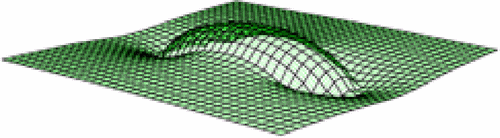
\includegraphics[scale = 0.5]{figures/literature_review/interfacial_curvature.png}
    \caption{Quadropolar capillary interactions around prolate ellipsoidal particles caused by interfacial deformations around the particle. 
    \cite{loudet_capillary_2005} Reproduced from Loudet et al. with license number RNP/25/FEB/088185}
    \label{fig:anisotropic_particle_interface}
\end{figure}

\section{Particle shape anisotropy and synthesis techniques}

Over the past decade, advancements in synthesis techniques have significantly expanded the ability to fabricate particles with anisotropic geometry and surface chemistry. 
The choice of synthesis method depends on the desired particle shape. For example, ellipsoidal particles can be readily produced through the mechanical deformation of 
polymer spheres, while dumbbell-shaped particles can be synthesized using microfluidic devices or emulsion templating. Square-shaped particles, on the other hand, can be 
generated through controlled crystallization \cite{morgan_understanding_2013}. The increasing variety of synthesis methods has reduced geometric constraints when exploring 
potential particle stabilizers for bijels \cite{wu_recent_2016}.

Anisotropic particles exhibit shape-dependent properties due to their ability to induce multipolar interactions by deforming the interface to maintain a mean curvature of 
zero, thereby satisfying the Young-Laplace equation, as illustrated in Figure \ref{fig:anisotropic_particle_interface} \cite{loudet_capillary_2005, cheng_shape-anisotropic_2013}.
This property has been leveraged to facilitate directed assembly and migration through modified capillary forces 
\cite{cavallaro_curvature-driven_2011, read_dimerization_2020, sharifi-mood_curvature_2015}.  

Anisotropic particles have also been shown to exhibit natural liquid crystal like behaviour as shown using Onsager theory. 

When stabilizing bijels, ellipsoidal particles provide greater stability than spherical ones due to their higher cross-sectional area-to-volume ratio, as demonstrated by 
Günther et al. and Hijnen et al. \cite{gunther_timescales_2014, hijnen_bijels_2015}. This enhanced stability arises from additional domain coarsening timescales associated 
with particle reorientation and increased mechanical rigidity, as confirmed by rheological studies \cite{gunther_timescales_2014, daware_emulsions_2015, witt_bijel_2013}. 
Furthermore, particle shape influences both the onset and dynamics of jamming. Studies using graphene plate-like particles have shown that these particles exhibit intrinsic 
elasticity, which affects the conditions under which jamming occurs \cite{imperiali_simple_2014, sun_assembly_2013}.

The orientation of ellipsoidal particles at interfaces is governed by a balance between interfacial capillary forces and external magnetic fields 
\cite{bresme_orientational_2007, davies_assembling_2014}. Theoretical studies and simulations suggest the existence of a critical field strength beyond which particle 
orientation is predominantly dictated by the applied field \cite{bresme_orientational_2007, davies_assembling_2014}. Additionally, both experimental and computational 
studies have shown that steric interactions—modulated by particle orientation and interfacial arrangements—play a significant role in determining the free energy of particle 
assemblies, underscoring the intricate interplay between these forces \cite{morgan_understanding_2013, newton_influence_2014, newton_capillary_2018}.

% The adsorption process is affected by the shape of particles used as they pack differently onto the interface \cite{hijnen_bijels_2015, daware_emulsions_2015,carmack_diverse_2017}. It has also been suggested that adsorption dynamics of ellipsoidal particles at liquid interfaces are driven completely by viscous forces even if the timescales of adsorption are driven by particle properties \cite{Coertjens2017}. Some guiding equations to calculate the interfacial area of an ellipsoidal particle are provided \cite{gunther_timescales_2014, Davies2014}.

\section{Bijel synthesis techniques}

The existence of bijels was first identified computationally using a multicomponent lattice boltzmann method which looked at 
the jamming of spherical particles in a binary fluid system with equal volume fraction of each fluid. 
\cite{stratford_colloidal_2005} Once phase separation was initiated, the particles adsorb onto the interface until the interfacial
area matches the cross sectional area of the particles at the interface, when domain coarsening is ceased. The simulation assumed
an equal volume fraction of fluid components and neutrally wetting particles to not impart preferential curvature onto the interface.
Figure \ref{fig:state_diagram_particle_emulsions} demonstrates a schematic derived from experimental results of particle stabilized
emulsion microstructures that form when changing the volume fraction and particle contact angle.

In experiments, bijels were first synthesized using Thermally Induced Phase Separation (TIPS) \cite{herzig_bicontinuous_2007, lee_bicontinuous_2010, bai_dynamics_2015}. 
The process begins by identifying a small-molecule or polymer blend with a critical point, referred to as the casting mixture, and preparing it at a composition 
corresponding to this critical point. The casting mixture is then combined with particle surfactants while remaining in a single-phase state. Once the particles 
are homogeneously distributed, phase separation is induced by adjusting the temperature to bring the system into the two-phase region. By ensuring that the 
composition aligns with the critical point, the casting mixture undergoes spinodal decomposition, preventing nucleation and growth. 

\begin{figure}
    \centering
    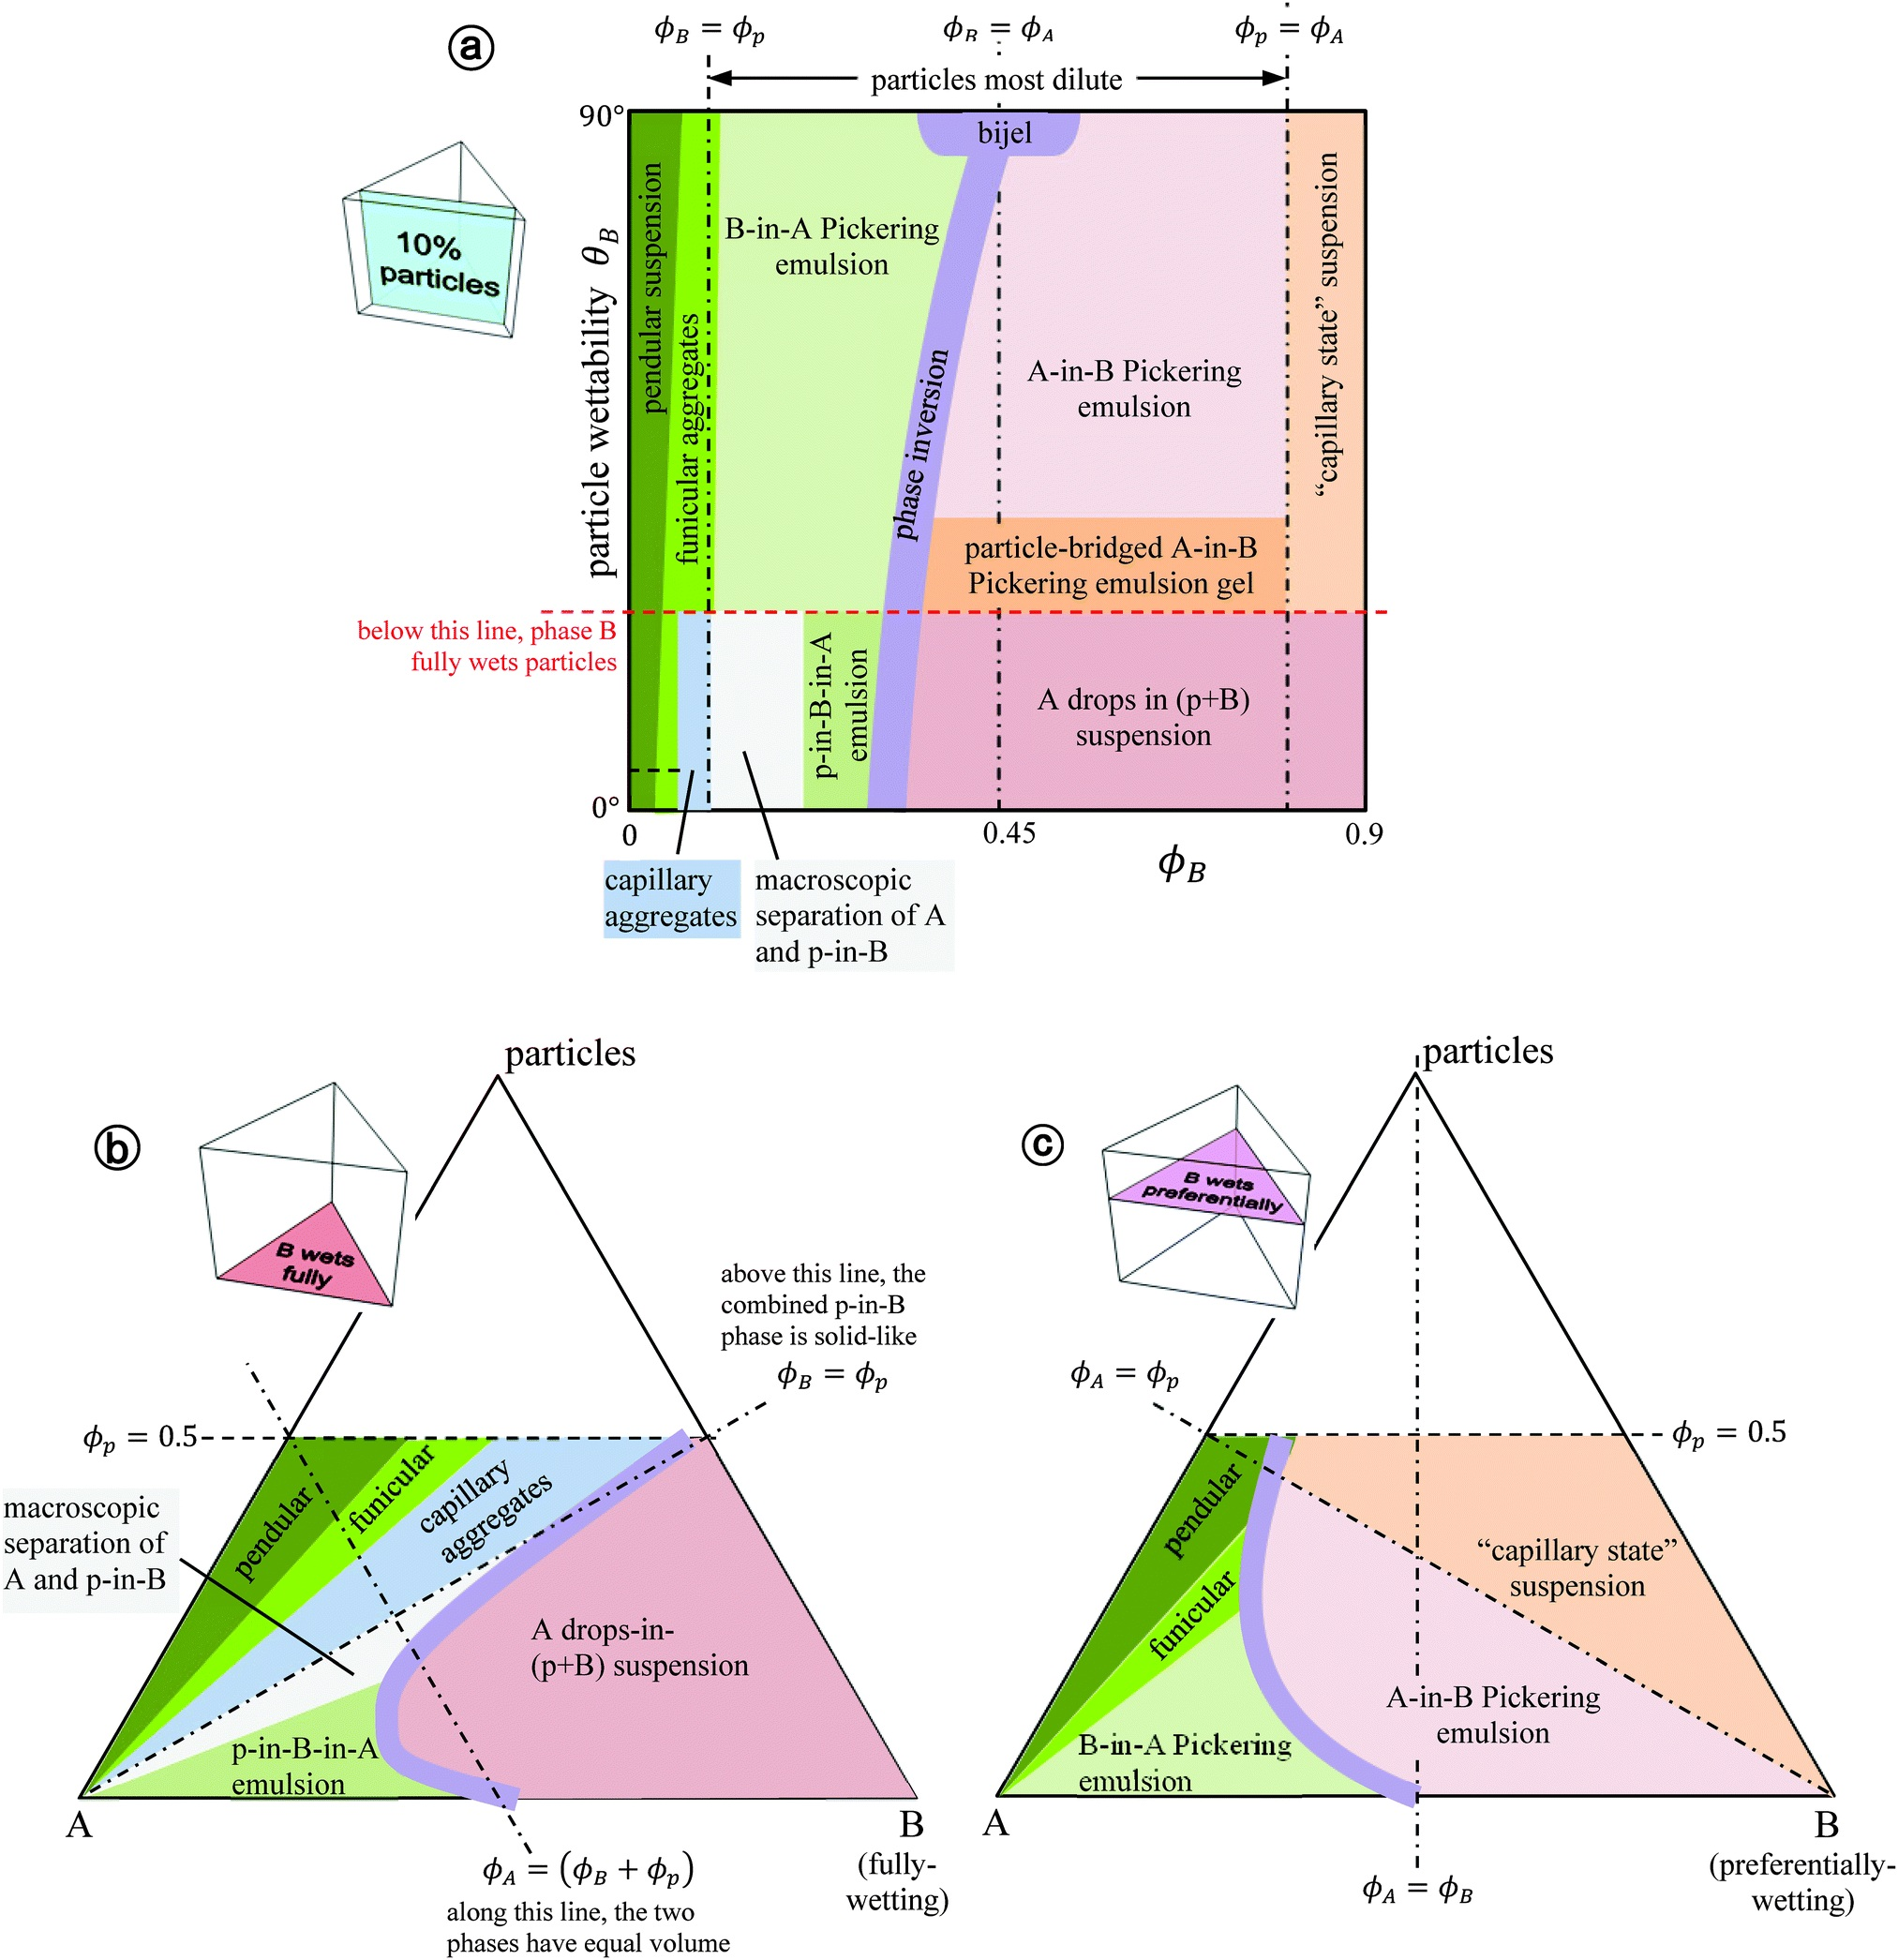
\includegraphics[scale = 0.2]{figures/literature_review/state_diagram.jpg}
    \caption{Formation criteria for a particle stabilized emulsion that can form bijel. 
            Reproduced from Velankar 2015 using license number 1551968-1. \cite{velankar_non-equilibrium_2015}}
    \label{fig:state_diagram_particle_emulsions}
\end{figure}

TIPS enables batch synthesis of bijels in research laboratories. However, for bijels to become industrially viable, a continuous fabrication process is required—one 
that also allows for the production of various bijel form factors suited to different applications. Solvent Transfer Induced Phase Separation (STrIPS) has been proposed 
as a method to achieve this. In STrIPS, a casting mixture is prepared, consisting of two fluids that form the bijel, a co-solvent, particles, and a surfactant. Phase 
separation is initiated as the co-solvent diffuses out of the bijel. The surfactant is included to maintain bijel stability against Marangoni forces. The casting mixture 
is then extruded into a bath of a non-solvent, which is immiscible with the bijel-forming fluids but miscible with the co-solvent. The diffusion of the co-solvent triggers 
phase separation, leading to bijel formation. The resulting microstructure is influenced by both the surfactant concentration and the flow rate of the casting mixture.

Vapor Induced Phase Separation(VIPS) has also been identified as a technique for continuous fabrication of bijels. \cite{wang_scalable_2020} A quarternary casting mixture
containing particles, solvent and two partially miscible liquids is prepared. The solvent and liquid species are carefully selected to ensure that removal of the
solvent will cause phase separation of the two partially miscible liquids. One system that has been used is the water/hexanediol-diacrylate solvated by ethanol.
Selection of the composition of the system facilitates crossing of the binodal through the critical point, causing phase separation through spinodal decomposition.
This technique has been used to fabricate thin films of bijels blade and spray coated onto substrates.

Instead of relying upon spinodal decomposition to generate the bijel morphology, homogenization uses shear to join phase separating domains, resulting in a 
structure that has the properties of a bijel even if not fabricated from fluids undergoing spinodal decomposition. \cite{huang_bicontinuous_2017, cai_bijels_2017} 
This method is primarily used for nanoparticles under $50$ nm and it has been shown to work for multiple particle geometries. This method relies upon
shear to cause limited coalescence of droplets. As coarsening occurs, particles adsorb on the interface and when the interfacial area matches the area of the
adsorbed particles, the microstructure jams. Tuning of the method can be done through modifying the contact angle of the particles at the interface as well as
the viscosity of the fluids. 

% \textcolor{blue}{Description of liquid in liquid printing}

% Enter something about this method. \cite{amirfattahi_fabrication_2024}

\section{Rheological models and shear response of bijels}

Bijels undergoing constant shear demonstrate shear thinning behavior which at moderate shear rates can be described reasonably well using the Herschel-Buckley
model. \cite{macmillan_rheological_2019, wang_morphology_2023} At higher shear rates, the bijel microstructure is destroyed and the viscosity becomes newtonian. 
\cite{cai_bijels_2017,bonaccorso_shear_2020}. Figure \ref{fig:bijel_under_shear} illustrates the findings of Bonnacorso et al., which observed that when a bijel 
stabilized with hard-sphere-like particles is subjected to shear, the particles initially align with the shear direction before detaching from the interface 
\cite{bonaccorso_shear_2020}. Investigating the impact of particle alignment on rheology, prior studies in suspension rheology have shown that colloidal systems 
with hard-sphere interparticle interactions undergoing constant shear exhibit shear banding—where particles order in the shear direction at moderate shear rates—resulting 
in shear thinning \cite{vermant_flow-induced_2005, brader_nonlinear_2010}. 

\begin{figure}
    \centering
    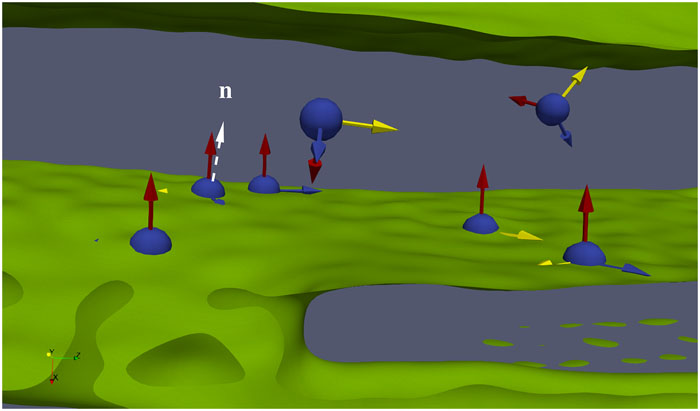
\includegraphics[scale = 2]{figures/literature_review/bijel_under_shear.jpeg}
    \caption{Schematic of a bijel with hard-sphere particles undergoing shear, demonstrating migration and detachment of particles at the interface. 
             Reproduced from Bonaccorso et al. under the Creative Commons CC BY License. \cite{bonaccorso_shear_2020}}
    \label{fig:bijel_under_shear}
\end{figure} 

Studies on complex bijel rheology have demonstrated gel-like characteristics when the storage modulus exceeds the loss modulus \cite{lee_making_2013, bai_dynamics_2015}. 
Ching and Mohraz further showed that the rheological behavior of bijels closely resembles that of a 2D colloidal glass percolating in 3D space, based on comparisons of 
linear viscoelasticity with colloidal gels composed of strongly attractive particles \cite{ching_bijel_2022}. Key characteristics of glasses include the presence of a 
yield stress, viscoelastic behavior, and a glass transition point \cite{pham_yielding_2008, weeks_introduction_2017}. Yield stress corresponds to the applied stress at 
which the particle monolayer undergoes irreversible structural changes \cite{pham_yielding_2008}. Viscoelasticity arises when the monolayer exhibits both solid and 
liquid-like behavior, depending on the timescale of the applied stress \cite{pham_yielding_2008}. The glass transition point is marked by a dramatic slowdown in the 
monolayer's dynamics \cite{weeks_introduction_2017}. 

% \textcolor{blue}{https://www.mdpi.com/2311-5521/5/3/150}

% \section{Colloidal glasses}

% \begin{itemize}
%     \item https://pubs.acs.org/doi/10.1021/acsmacrolett.6b00826
%     \item Add stuff on dynamic heterogeneity
%     \begin{itemize}
%         \item https://pubs.rsc.org/en/content/articlelanding/2012/sm/c2sm25267h
%     \end{itemize}
%     \item Add stuff on particle jamming
%     \begin{itemize}
%         \item https://journals.aps.org/rmp/pdf/10.1103/RevModPhys.82.2633
%     \end{itemize}
%     \item Add stuff on cooperatively rearranging regions
%         \begin{itemize}
%             \item https://doi.org/10.1038/ncomms4829
%             \item https://journals.aps.org/prl/abstract/10.1103/PhysRevLett.110.188301
%             \item https://journals.aps.org/prl/abstract/10.1103/PhysRevLett.107.065702
%         \end{itemize}
%     \item Add stuff on reentrant glass phenomena 
%     \begin{itemize}
%         \item https://doi.org/10.1209/0295-5075/86/58001
%     \end{itemize}
% \end{itemize}

\section{Microstructure control in bijels}

Kim et al. used a free energy based lattice boltzmann method coupled with particles and magnetic fields to investigate the influence of magnetic fields on 
the microstructure of bijels stabilized with spherical particles. \cite{kim_bijels_2010}
They observed that applying strong magnetic fields did not significantly alter the bijel microstructure, as the particles aligned with 
the field without disrupting the interfacial ordering. This finding suggests that spherical particles, due to their isotropic shape, do 
not induce anisotropic stresses on the interface when subjected to magnetic fields, thereby maintaining the structural integrity of the bijel.

In contrast to the minimal impact of magnetic fields on bijels stabilized with spherical particles, Carmack and Millett investigated the effects of 
applied electric fields on thin-film bijels using a Cahn-Hilliard coupled with Langevin dynamics computational model. \cite{carmack_tuning_2018} 
Their study revealed that electric fields can induce significant microstructural changes in bijels, with particles self-assembling into chains and forming 
cylindrical domains aligned parallel to the applied field, thereby modifying the overall microstructure. Carmack and Millet observed that the dielectric contrast 
between liquid domains governs liquid domain alignment, and the dielectric contrast between colloidal particles and the liquid matrix induces dipolar particle 
interactions. By changing the dielectric contrast between particle and fluid, different bijel morphologies could be formed. Additionally, particle chains were found to 
act as nucleation sites for phase separation, influencing the resultant morphologies in terms of particle attachment to phase interface regions and average 
channel diameter. 

While not strictly stimuli-responsive, microstructure modifications have been achieved by applying a particle volume fraction gradient during the formation of 
bijels using Thermally Induced Phase Separation (TIPS). \cite{french_bicontinuous_2022} In their study, French et al. allowed particles to partially sediment in the bijel casting mixture
before initiating thermal quenching. The gradient in particle volume fraction along the height of the reaction vessel caused the jamming point of the bijel
to vary along the gradient axis, causing a channel size gradients of up to 2.8\% per millimeter, as measured using confocal microscopy.

\section{Lattice Boltzmann Method}

The Lattice Boltzmann Method (LBM) is an evolution of preceding lattice gas automata techniques, which is a discretization of the Boltzmann equation of motion for 
molecules. This means that unlike traditional CFD techniques such as FDM, VOF or level set methods, LBM is a psuedo-molecule method that tracks the evolution of a 
particle distribution function within grid cells evolved through a discretized Boltzmann equation of motion. Macroscopic variables such as fluid density and 
velocity are recovered from the particle distributions through appropriate moment integration, and the Navier Stokes equation at the incompressible limit can be 
obtained through a Chapman-Enskog expansion of the LBM. The LBM has become an attractive tool for meso-scale CFD simulations due to its ease of algorithm 
implementation, highly parallelizable nature and ease of boundary condition implementation, allowing coupling to other physically relevant systems such as 
particles with varieties of potentials, external fields and deformable bodies.

The particle distribution function described earlier is advected on a pre-constructed lattice stencil, commonly denoted as DnQm where n and m represent the 
number of dimensions and directions in the stencil. Common stencils include the D1Q5, D2Q9 and D3Q19 stencil, all of which recover mass and momentum conservation. 
For energy conservation, a higher order stencil such as D3Q27 is necessary. The D2Q9 and D3Q19 stencils have 8 and 18 populations respectively that include 
connections to nearest and next nearest neighbour points, in addition to a central rest point. 

The LBM is composed of a collision and advection step. In the advection step, the populations at each grid point are propagated to adjacent points in accordance 
with the chosen stencil. During the collision step, the particle population distribution is relaxed towards an equilibrium with a collision operator, at a 
specified relaxation rate. The collision operator can have multiple forms based on how many relaxation rates are used although the most common variant is the 
Single Relaxation Time (SRT) collision operator, more commonly known as the Bhatnagar-Gross-Krook (BGK) collision operator. Owing to its stability in low Mach 
and Reynolds numbers and simplicity of implementation, the BGK operator is often used in common particle laden flow and soft matter scenarios. 
\cite{bhatnagar_model_1954} These limitations are present owing to the implicit link between the fluid properties and the relaxation rate necessitating 
relaxation rates above 0.5, and to ensure fluid incompressibility from an equation that intrinsically simulates a compressible fluid. To get over these 
limitations, Two Relaxation Time (TRT) and Multiple Relaxation Time (MRT) operators also exist, expanding the possible application of the LBM to visco-elastic 
flows and implementation of fluctuating hydrodynamics in the LBM. \cite{liu_simulation_2023, adhikari_fluctuating_2005}

Four primary techniques to model multicomponent or multiphase systems exist in the LBM literature. A quick review of the Shan-Chen or 
interparticle potential model  will be provided here from the perspective of a binary mixture. Additionally, the names and descriptions of 
other techniques will be described as well. The interparticle potential model or Shan-Chen model that adds a non-local density dependent force 
between two species, effectively modelling non-ideal mixing and recovering the Cahn-Hilliard equation. To alleviate the standard Shan-Chen implementations 
weaknesses of not being thermodynamically consistent and reducing the existence of spurious velocities, 

In addition to the Shan-Chen model, the color gradient model, free energy model and interface tracking technique all 
allow for simulations of various types of multiphase and/or multicomponent flows. The color gradient model proposed by Rothman and Keller and 
implemented by Gunstensen et al relies upon modelling two particle distributions. These represent a binary fluid mixture with the collision step 
able to recover the hydrodynamics and non-ideal mixing dynamics. The free energy model utilizes phase field theory and constructs a free energy 
functional to recover interfacial dynamics and effects in a thermodynamically consistent manner. Often, a square gradient free energy is used for 
simplicity and ease of implementation. The mean field theory The non-ideal mixing dynamics are recovered during the "recoloring" step, of which the 
technique proposed by Latva-Kokko and Rothman is more commonly used for soft matter flows. \cite{liu_multiphase_2016}